\documentclass[12pt, letterpaper]{article}
\usepackage[utf8]{inputenc}

\usepackage{setspace}
\onehalfspacing

\makeindex
\usepackage{textcomp}
\usepackage{float}
\usepackage{fancyhdr}
\usepackage{makeidx}
\pagestyle{myheadings}
\fancyhf{}
\rhead[\leftmark]{thepage}
\usepackage[toc,page]{appendix}

\usepackage[T1]{fontenc}
\usepackage[utf8]{inputenc}
\usepackage{url}
\setlength {\marginparwidth}{2cm}
\usepackage{todonotes}

\usepackage[all]{xy}
\usepackage{graphicx}
\usepackage{units}
\usepackage{enumerate}
\usepackage[hidelinks]{hyperref}
\usepackage[]{algorithm2e} %algorithm


\usepackage{amssymb, amsmath, amsthm, pict2e}
 \pagestyle{myheadings}

\usepackage{pdfsync}
\usepackage{rotating}
\usepackage{multirow}
\usepackage[normalem]{ulem}
\usepackage{cancel}

\usepackage{color}
%\usepackage[usenames,dvipsnames,svgnames,table]{xcolor}
\usepackage{pgf,tikz}
\usetikzlibrary{decorations,arrows}
%\usetikzlibrary{decorations.pathmorphing}
\usepgflibrary{decorations.pathreplacing}

\def\arr{\hbox{𝓇}}

\usepackage{environ}
\makeatletter
\newsavebox{\measure@tikzpicture}
\NewEnviron{scaletikzpicturetowidth}[1]{%
  \def\tikz@width{#1}%
  \def\tikzscale{1}\begin{lrbox}{\measure@tikzpicture}%
  \BODY
  \end{lrbox}%
  \pgfmathparse{#1/\wd\measure@tikzpicture}%
  \edef\tikzscale{\pgfmathresult}%
  \BODY
}

%%%%%%%%%%%%%%%%  start macros  %%%%%%%%%%%%%%%%%%%%%%%%%%%%%%%%%
\newtheorem{theorem}{Theorem}
\theoremstyle{definition}
\newtheorem{defn}[theorem]{Definition}
\newtheorem{example}[theorem]{Example}
\theoremstyle{remark}
\newtheorem{remark}[theorem]{Remark}
\newtheorem{question}[theorem]{Question}

\theoremstyle{plain}
\newtheorem{lemma}[theorem]{Lemma}
\newtheorem{claim}[theorem]{Claim}
\newtheorem{obs}[theorem]{Observation}
\newtheorem{prop}[theorem]{Proposition}
\newtheorem{corollary}[theorem]{Corollary}
\newtheorem{conjecture}[theorem]{Conjecture}

\newtheorem{hyp}[theorem]{Hypothesis}
\newtheorem{alg}[theorem]{Algorithm}
\numberwithin{theorem}{section}
\newcommand{\powerset}{\raisebox{.15\baselineskip}{\Large\ensuremath{\wp}}}

%\newcommand{\qed}{\mbox{$\Box$}}
%\newcommand{\proof}{\medbreak\par\noindent{\bf Proof. }}
\newtheorem{proofpart}{Part}
\makeatletter
\@addtoreset{proofpart}{theorem}
\makeatother
 \newcommand{\GP}{{\vec{G}}_P}
\newcommand{\GN}{{\vec{G}}_N}

\newcommand{\cover}{\mathrel{\rlap{$\prec$}
                                \rlap{\hskip 0.7em $\cdot$}
                                 \phantom{\prec}}}

\newcommand{\re}{re}

\newcommand{\up}{\mbox{\rm{up}}}
\newcommand{\side}{\mbox{\rm{side}}}
\newcommand{\type}{\mbox{\rm{type}}}


\def\reals{{\mathbb R}}


\newcommand{\ahat}{{\hat{a}}}
\newcommand{\bhat}{{\hat{b}}}
\newcommand{\chat}{{\hat{c}}}
\newcommand{\dhat}{{\hat{d}}}
\newcommand{\bolda}{{\bf{a}}}
\newcommand{\boldb}{{\bf{b}}}
\newcommand{\boldc}{{\bf{c}}}
\newcommand{\boldd}{{\bf{d}}}

\newcommand{\iplus}{{\cal I}^+}
\newcommand{\iminus}{{\cal I}^-}
\newcommand{\ipm}{{\cal I}^{\pm}}
\newcommand{\ipmix}{{\cal I}^{{\cal M}}}

\newcommand{\upl}{{\cal U}^+}
\newcommand{\uminus}{{\cal U}^-}
\newcommand{\upm}{{\cal U}^{\pm}}
\newcommand{\upmix}{{\cal U}^{{\cal M}}}


\newcommand{\ppl}{{\cal P}^+}
\newcommand{\pminus}{{\cal P}^-}
\newcommand{\ppm}{{\cal P}^{\pm}}
\newcommand{\ppmix}{{\cal P}^{{\cal M}}}
\newcommand{\bpm}{{\cal B}^{\pm}}
\newcommand{\tpm}{{\cal T}^{\pm}}
\newcommand{\bpmix}{{\cal B}^{{\cal M}}}
\newcommand{\tpmix}{{\cal T}^{{\cal M}}}
%%%%%%%%%%%%%%%%  end macros  %%%%%%%%%%%%%%%%%%%%%%%%%%%%%%%%%


\parindent1em
%\parskip1.0ex

\title{Coordinates of $K_{1,3}$ in TSG}
\author{Abdeselam El-Haman Abdeselam}
\date{June 6th, 2019}

\begin{document}

\begin{figure}
\centering

\begin{scaletikzpicturetowidth}{\textwidth}
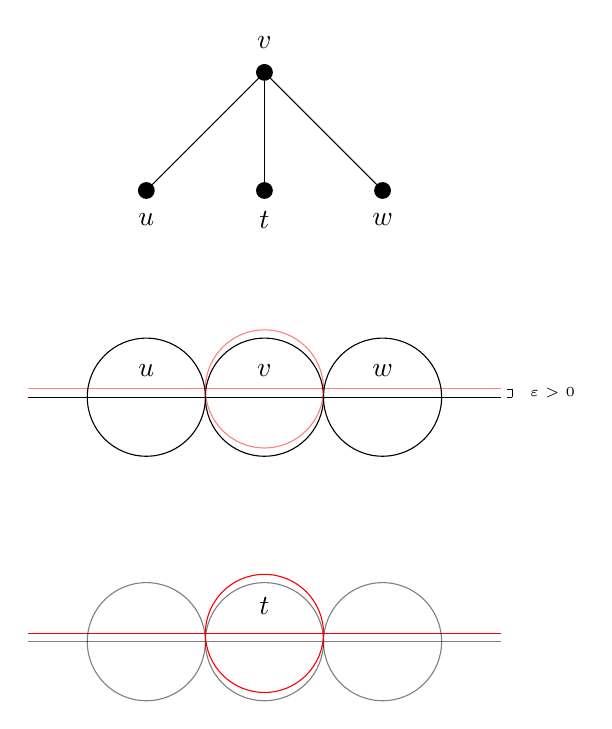
\begin{tikzpicture}[scale=1.5]

\draw (-2,0) -- (2,0);
\draw[red ,opacity = 0.5] (-2,0.07) -- (2,0.07);
\draw  (-1,0) circle [radius=0.5];
\draw[color=black] (-1,0.2265) node {$u$};
\draw  (0,0) circle [radius=0.5];
\draw[color=black] (0,0.2265) node {$v$};
\draw  (1,0) circle [radius=0.5];
\draw[color=black] (1,0.2265) node {$w$};

\draw[red, opacity = 0.5] (0,0.07) circle [radius=0.5];
\draw[color=black] (2.4386,0.0367) node {\tiny $\varepsilon > 0$};

% lines to describe distance (epsilon)
\draw[very thin] (2.1,0.07) -- (2.1,0);
\draw[very thin] (2.05,0.07) -- (2.1,0.07);
\draw[very thin] (2.05,0) -- (2.1,0);

\draw[opacity = 0.5] (-2,-2.07) -- (2,-2.07);
\draw[red] (-2,-2) -- (2,-2);
\draw[opacity = 0.5]  (0,-2.07) circle [radius=0.5];
\draw[opacity = 0.5]  (1,-2.07) circle [radius=0.5];
\draw[opacity = 0.5]  (-1,-2.07) circle [radius=0.5];
\draw[red] (0,-2) circle [radius=0.5];
\draw[color=black] (0,-1.765) node {$t$};

\node[draw,circle,inner sep=2pt,fill,label distance=1cm] (v1) at (0,2.75) {};
\draw[color=black] (0,3) node {$v$};
\node[draw,circle,inner sep=2pt,fill,label distance=1cm] (v3) at (0,1.75) {};
\draw[color=black] (0,1.5) node {$t$};
\node[draw,circle,inner sep=2pt,fill,label distance=1cm] (v2) at (-1,1.75) {};
\draw[color=black] (1,1.5) node {$w$};
\node[draw,circle,inner sep=2pt,fill,label distance=1cm] (v4) at (1,1.75) {};
\draw[color=black] (-1,1.5) node {$u$};
\draw  (v1) edge (v2);
\draw  (v1) edge (v3);
\draw  (v1) edge (v4);
\end{tikzpicture}
\end{scaletikzpicturetowidth}
\caption{$K_{1,3}$ with its unique thin strip graph realization.}
\label{fig:thinK13}
\end{figure}

\begin{lemma}
  The only way to represent $K_{1,3}$ as a thin strip graph is for three points $u,v,w$ such that $u_x=v_x-1$ and $w_x = v_x+1$ with the same
  $y$-coordinate and the fourth point $t$ is placed such $t_x = v_x$ and $t_y \neq v_y$ (see Figure \ref{fig:thinK13}).
\end{lemma}

\proof{
We proceed to prove this lemma by contradiction. We begin constructing the realization of $K_{1,3}$ by taking its induced $P_3 \in K_{1,3}$. The middle point of $P_3$ has to be between
the other two points horizontally, so we know then that $u_x < v_x < w_x$ with $v$ the middle point.\\

Now we introduce $t$, the vertex that is adjacent to the middle point of $P_3$. We know by fact that $u_x < t_x < w_x$: if we take $t_x \leq u_x$, $t$ has to be adjacent to $u$ in order to intersect $v$ which is not the case; viceversa for $w$.

Let $\alpha_{u,v} = \sqrt{1 - (u_y-v_y)^2}$ be a real number that represents the \emph{critical region} between two points.
Note that if $|u_x - v_x| \leq \alpha_{u,v}$ then $u$ and $v$ are intersecting and $0 < \alpha_{u,v} < 1$.

Now that we know that $u_x < t_x < w_x$, if we set $t_x < v_x$ and maximize the distance between $u$ and $v$ (so $u_x = v_x-1$) we should have:

$$t_x > \alpha_{u,t}+u_x$$

for every $t_y$. We assume that $v_y = 0$ and $v_x = k$ with $k \in \mathbb{R}$ without loss of generality.


\begin{equation*}
  \begin{split}
    & t_x > \alpha_{u,t}+v_x-1\\
    & v_x > t_x > \alpha_{u,t}+v_x-1\\
    & 0 > \alpha_{u,t}-1\\
    & 1 > \alpha_{u,t}
  \end{split}
\end{equation*}

Which is impossible because $t$ and $u$ are non-adjacent vertices which means that $\alpha_{u,t}$ has to be bigger than one by the definition of $\alpha_{u,t}$. The same occurs with $w_x$ and $t_x > v_x$.

The only case left is when $t_x = v_x$. If $u$ and $t$ intersect then:

\begin{equation*}
  \begin{split}
&t_x \leq \alpha_{u,t}+u_x\\
&t_x+1 \leq \alpha_{u,t}+v_x
\end{split}
\end{equation*}

we know that $t_x = v_x$ and $v_y = u_y = 0$ without loss of generality:

\begin{equation*}
  \begin{split}
    v_x+1 & \leq \alpha_{u,t}+v_x\\
    1 & \leq \alpha_{u,t}\\
    & \leq \sqrt{1-t_y^2}
\end{split}
\end{equation*}
which is impossible except when $t_y = 0$. The same happens when we suppose that $t$ and $w$ intersect.\\

Finally, we have to prove that the assumption of maximality $u_x = v_x-1$ and $w_x = v_x+1$ are the only solutions for this graph. By symmetry, we only have to prove this for $u$.

Let $u_x < v_x-1$. In this case, $u$ and $v$ are not adjacent because $|u_x - v_x| > 1 > \alpha_{u,v}$. Otherwise, if $u_x > v_x-1$ and we know that $t_x = v_x$, we can state that $u_x - k = v_x-1$ where $0 < k < 1$ is a positive real number. We have to see if there always exists a value of $t_y > 0$ for every $k$ so that $u$ and $t$ are adjacent to each other.

\begin{equation*}
  \begin{split}
    u_x - k &= t_x - 1\\
    t_x - u_x &= 1 - k \leq \alpha_{u,t}\\
    1 - k &\leq \sqrt{1 - t_y^2}\\
    (1 - k)^2 &\leq 1 - t_y^2\\
    k^2 -2k +1 &\leq 1 - t_y^2\\
    2k-k^2 &\geq t_y^2\\
    \sqrt{2k-k^2} &\geq t_y
  \end{split}
\end{equation*}

We know that $\sqrt{2k-k^2} > 0$, so we always have a $t_y$ such that $\sqrt{2k-k^2} > t_y > 0$. This is a contradiction to the main proposition because $u$ and $t$ do not have to be adjacent to each other despite of the last equation which shows us that for every deplacement to the right of $u$, there will always a $t_y$-strip graph for which $u$ and $t$ will be adjacent given if $u_x > t_x-1$.\\

This means that the only solutions are when $t_y \neq v_y$, $t_x = v_x$, $u_x = v_x-1$, $w_x = v_x+1$ and $v_y = u_y = w_y$. \qed
}
\end{document}
